\documentclass[12pt,a4paper]{article}
\usepackage{amsmath,amsfonts,amsthm,amssymb}
\usepackage{physics}
\usepackage{geometry}
\usepackage{graphicx}
\usepackage{setspace}
\doublespacing{}
\title{Angles}
\author{}
\date{}

\begin{document}

\maketitle

\section{Definition}
In Euclidean geometry, an angle is the figure formed by {\bf two rays}, 
called the sides of the angle, sharing a common endpoint, 
called the {\bf vertex} of the angle. 
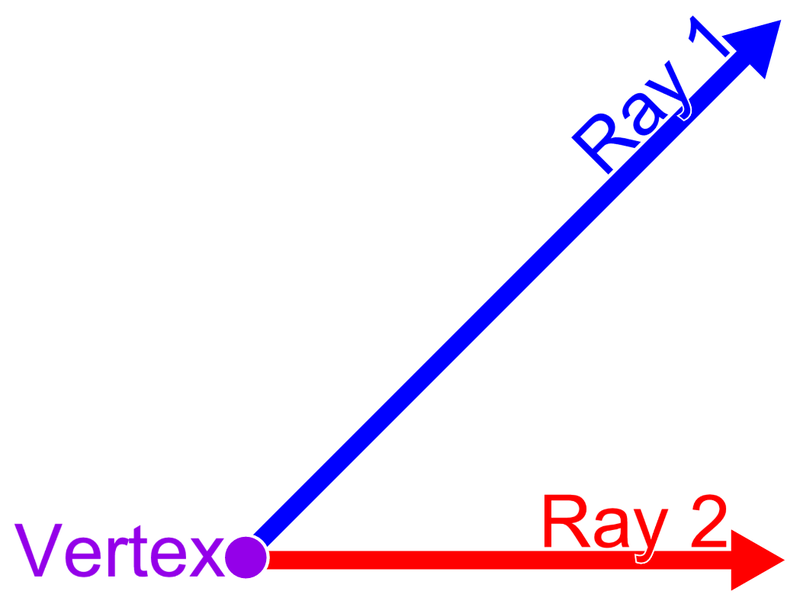
\includegraphics[width=0.9\textwidth]{ray.png}

\section{Types}
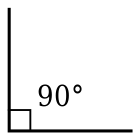
\includegraphics[width=0.2\textwidth]{right.png}
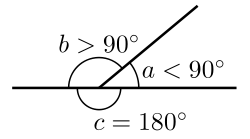
\includegraphics[width=0.5\textwidth]{angles.png}
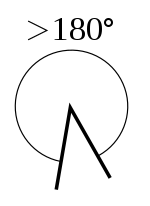
\includegraphics[width=0.2\textwidth]{reflex.png}
\begin{itemize}
    \item an angle of \(0^\circ<a<90^\circ\) is called an {\bf acute angle}
    \item an angle of \(90^\circ\) is called a {\bf right angle}
    \item an angle of \(90^\circ<b<180^\circ\) is called an {\bf obtuse angle}
    \item an angle of \(c=180^\circ\) is called a {\bf straight angle}
    \item an angle of \(>180^\circ\) is called a {\bf reflex angle}
    \item an angle of \(360^\circ\) is called a {\bf complete turn}
\end{itemize}

\newpage

\section{Adjacent Angle Pairs}
Two angles are {\bf adjacent angles} if and only if:
\begin{itemize}
    \item they share a common vertex and a common ray, AND
    \item they lie on the opposite sides of the common ray
\end{itemize}
\begin{center}
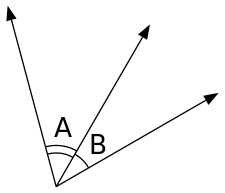
\includegraphics[width=0.5\textwidth]{adjacent.png}
\end{center}
Angles \(A\) and \(B\) are adjacent angles.

\newpage

\section{Combining Angle Pairs}
\subsection{Complementary Angles}
Two angles are said to be {\bf complementary angles} if their sum is \(90^\circ\).
\begin{center}
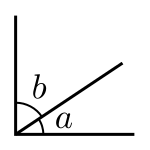
\includegraphics[width=0.4\textwidth]{complementary.png}
\end{center}
Since \(a+b=90^\circ\), \(a\) and \(b\) are complementary.
\subsection{Supplementary Angles}
Two angles are said to be {\bf supplementary angles} if their sum is \(180^\circ\).
\begin{center}
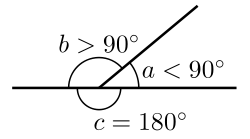
\includegraphics[width=0.5\textwidth]{angles.png}
\end{center}
Since \(a+b=180^\circ\), \(a\) and \(b\) are supplementary.

\section{Equivalence Angle Pairs}
\subsection{Vertically Opposite Angles}
When two straight lines intersect at a point, four angles are formed. 
Pairwise these angles are named according to their location 
relative to each other.
Vertically opposite angles are {\bf equal in size}.
\begin{center}
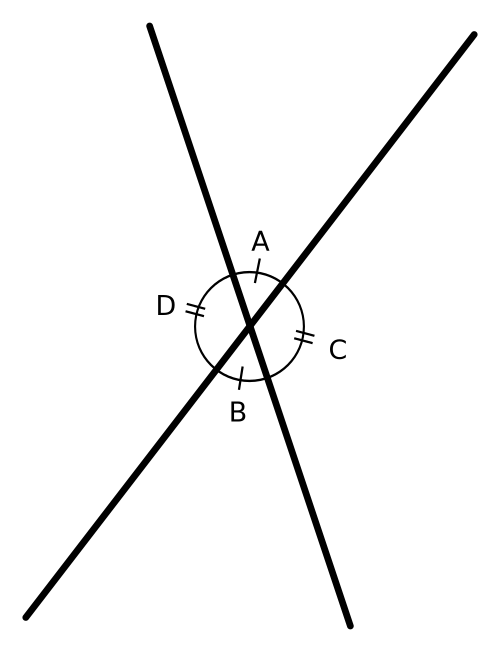
\includegraphics[width=0.5\textwidth]{Vertical_Angles.png}
\end{center}
There are 2 pairs of vertically opposite angles. 
One pair is \(A\) and \(B\). The other pair is \(C\) and \(D\).
\newpage
\subsection{Angles at a Point}
\(A\), \(B\), \(C\) and \(D\) are also called angles at a point. 
Angles at a point add up to one turn.
\begin{center}
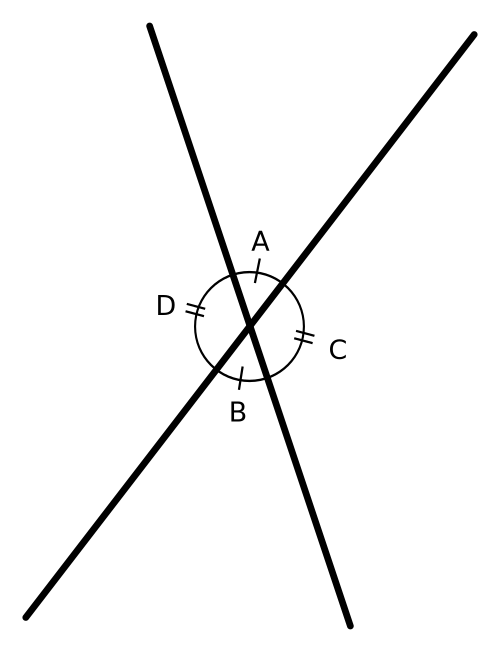
\includegraphics[width=0.5\textwidth]{Vertical_Angles.png}
\end{center}
In this case, \(A+B+C+D=360^\circ\).

\newpage
\section{Parallel Lines and Angles of a Transversal}
\subsection{Parallel Lines}
{\bf Parallel lines} are the straight lines that never intersect.
In geometry, we use a pair of arrows to indicate parallel lines.
\begin{center}
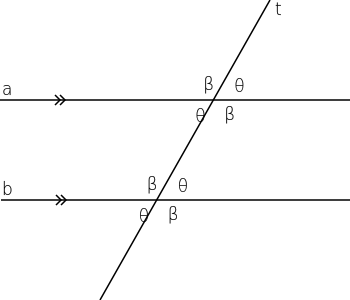
\includegraphics[width=0.5\textwidth]{pl.png}
\end{center}
Lines \(a\) and \(b\) are parallel.
This relationship can be expressed as \(a\parallel b\).
\newpage
\subsection{Corresponding Angles}
Two angles are said to be {\bf corresponding angles} if they have the same relative 
positive at the each intersection where
a line, called a transversal, cuts across a pair of parallel lines. 
The corresponding angles are equal to each other. 
\begin{center}
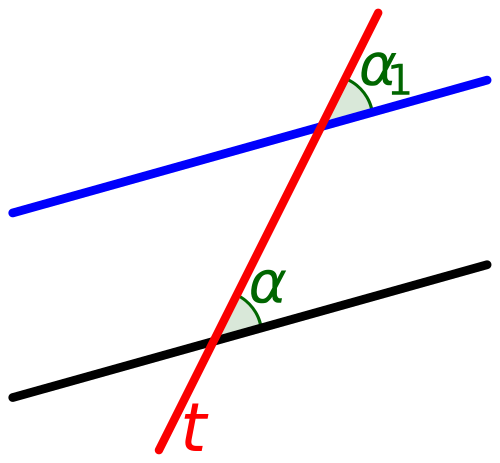
\includegraphics[width=0.5\textwidth]{corr.png}
\end{center}
In this case, line \(t\) is the transversal with
\(\alpha\) and \(\alpha_1\) begin a pair of 
corresponding angles. This means \(\alpha_1=\alpha\).
\newpage
\subsection{Alternate Angles}
Two angles are called {\bf alternate angles}
if they lie on the different side of the transversal.
The alternate angles are equal to each other. 
\begin{center}
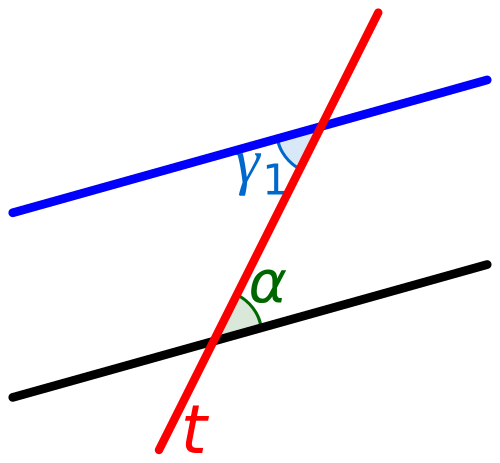
\includegraphics[width=0.5\textwidth]{alt.png}
\end{center}
In this case, line \(t\) is the transversal with
\(\alpha\) and \(\gamma_1\) begin a pair of 
alternate angles. This means \(\gamma_1=\alpha\).
\newpage
\subsection{Consecutive Interior Angles}
Two angles are known as {\bf interior angles}
if they lie on the same side of the transversal.
The interior angles are {\bf supplementary}. 
\begin{center}
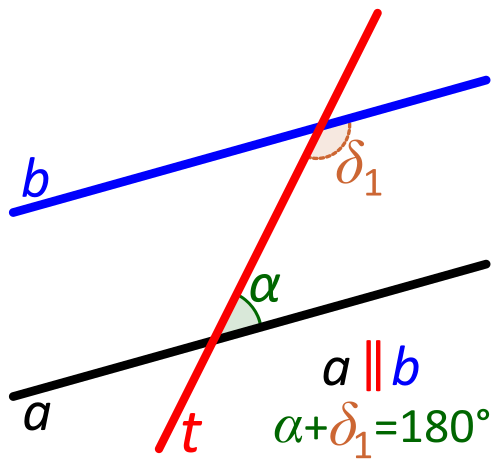
\includegraphics[width=0.5\textwidth]{int.png}
\end{center}
In this case, line \(t\) is the transversal with
\(\alpha\) and \(\delta_1\) begin a pair of 
interior angles. This means \(\alpha+\delta_1=180^\circ\).
\end{document}
